\documentclass[../calc1-main.tex]{subfiles}

\begin{document}

  An \textbf{exponential function} is a function of the form $f(x) = a^x$ where the \textbf{base} $a$ is a positive constant and the \textbf{exponent} $x$ is the variable. Let's define this function.

  \begin{itemize}
    \item $a^0 = 1$.
    \item $a^n = a \cdot a \cdots a$ (n -times) if $n = 1, 2, 3, \dots$.
    \item $a^{-n} = \frac{1}{a^n}$ if $n=1, 2, 3, \dots$.
    \item $a^{m/n} = \sqrt[n]{a^m}$ if $n=1, 2, \dots$ and $m = \pm 1, \pm 2, \dots$.
  \end{itemize}

  How should we define $a^x$ if $x$ is not rational? What does $2^{\pi}$ mean? We will define $a^x$ for irrational $x$ in the next section. For now, let us regard $a^x$ as a limit as discussed in the next problem.

  \begin{example}
    Since the irrational number $\pi = 3.141592\dots$ is the limit of the sequence of rational numbers
    \[
      r_1 = 3 \quad r_2 = 3.1 \quad r_3 = 3.14 \quad \dots
    \]
    we can calculate $2^{\pi}$ as the limit of the sequence
    \[
      2^3 = 8 \quad 2^{3.1} = 8.5741877\dots \quad 2^{3.14} = 8.8152409\dots
    \]
    This gives
    \[
      2^{\pi} = \lim_{n \to \infty} 2^{r_n} = 8.824977\dots
    \]
  \end{example}
  If $x$ is irrational, then we define $a^x$ as the limit values $a^r$ for rational numbers $r$ approaching $x$
  \[
    a^x = \lim_{\substack{r \to x \\ \text{r is rational}}} a^r. \qquad
  \]

  \textbf{Laws of Exponents}

  If $a>0$ and $b>0$ and $x$, $y$ are real numbers then
  \begin{multicols}{2}
    \begin{enumerate}
      \item $a^{0} = 1$,
      \item $a^{x+y} = a^x a^y$,
      \item $a^{-x} = \dfrac{1}{a^x}$,
      \item $a^{x-y} = \dfrac{a^x}{a^y}$,
      \item $(a^x)^y = a^{xy}$,
      \item $(ab)^x = a^x b^x$.
    \end{enumerate}
  \end{multicols}

  If $a>1$ then
  \[
    \lim_{x \to \infty} a^x = \infty, \qquad
    \lim_{x \to -\infty} a^x = 0.
  \]

  If $0<a<1$ then
  \[
    \lim_{x \to \infty} a^x = 0, \qquad
    \lim_{x \to -\infty} a^x = \infty.
  \]
  The domain of $a^x$ is $(-\infty, \infty)$ and its range is $(0, \infty)$.
  \begin{figure}[H]
    \centering
    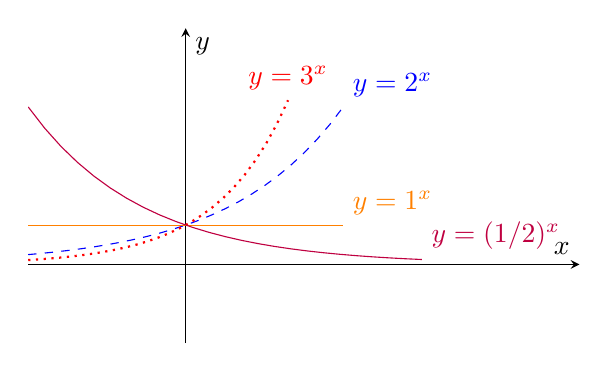
\begin{tikzpicture}
  \begin{axis}[
  x=10mm, y=5mm,
  xmax=5, ymax=6, ymin=-2,
  ticks=none,
  xlabel=$x$, ylabel=$y$,
  axis lines=middle]
  \addplot[blue, dashed, domain=-2:2]  {pow(2,x)} node[above right]{$y=2^x$};
  \addplot[red, dotted, thick, domain=-2:1.3]  {pow(3,x)} node[above]{$y=3^x$};
  \addplot[orange, domain=-2:2]  {1} node[above right]{$y=1^x$};
  \addplot[purple, domain=-2:3]  {pow(.5, x)} node[above right]{$y=(1/2)^x$};
\end{axis}
\end{tikzpicture}
  \end{figure}

  \subsection*{Logarithm}

  If $a >0$ and $a \neq 1$ then the function $a^x$ is 1-1 ($1^x$ has no inverse). The inverse function of $a^x$ is $\log_a x$, called the \textbf{logarithm of $x$ base $a$}.
  \[
    y = \log_a x \iff x = a^y
  \]

  Since $a^x$ has domain $(-\infty, \infty)$, and range $(0, \infty)$, $\log_a x$ has domain $(0, \infty)$ and range $(-\infty, \infty)$.

  Since $a^x$ and $\log_a x$ are inverse functions
  \[
    \log_a a^x = x \quad \forall x, \qquad a^{\log_a x} = x, \quad x>0
  \]

  \begin{figure}[H]
    \centering
    \begin{tikzpicture}
  \begin{axis}[
  xlabel=$x$, ylabel=$y$,
  xmin=-3, xmax=12, ymax=12, ymin=-3,
  ticks=none,
  axis lines=middle]
  \addplot[red, domain=-2:3]  {pow(2,x)} node[above]{$y=a^x$};
  \addplot[black, domain=-5:10]  {x} node[above]{$y=x$};
  \addplot[purple, domain=1/2^6:10,samples=100]  {log2(x)} node[above left] {$y=\log_a x$};
\end{axis}
\end{tikzpicture}
    \caption{The graph of logarithmic function is a reflection of the graph of the exponential function in the line $y = x$.}
  \end{figure}

  \textbf{Laws of Logarithm}
  If $x>0$, $y>0$, $a>0$, $b>0$, $a \neq 1$, $b \neq 1$, then

  \begin{multicols}{2}
    \begin{enumerate}
      \item $\log_a 1 = 0$
      \item $\log_a (x y) = \log_a x + \log_a y$
      \item $\log_a (\dfrac{1}{x}) = - \log_a x$
      \item $\log_a (\dfrac{x}{y}) = \log_a x - \log_a y$
      \item $\log_a x^y = y \log_a x$
      \item $\log_a x = \dfrac{\log_b x}{\log_b a}$
    \end{enumerate}
  \end{multicols}

  \begin{example}
    Prove $\log_a (x y) = \log_a x + \log_a y$ using laws of exponent.
  \end{example}
  \begin{solution}
    Take $u = \log_a x$, $v = \log_a y$ then $x = a^u$, $y = a^v$ and
    \[
      x y = a^{u+v} \iff u + v = \log(xy)
    \]
  \end{solution}

  \begin{example}
    Simplify
    \begin{enumerate}
      \item $\log_2 10 + \log_2 12 - \log_2 15$.
      \[
        \log_2 10 + \log_2 12 - \log_2 15
        = \log_2 \frac{10 \times 12}{15} = \log_2 8 = 3
      \]
      \item $\log_{a^2} a^3$.
      \[
       \log_{a^2} a^3
       = \frac{\log_a a^3}{\log_a a^2} = \frac{3}{2}
     \]
     \item $3^{\log_9 4}$.
     \[
      3^{\log_9 4}
      = 3^{\frac{1}{2} \log_3 4} = 3^{\log_3 2} = 2
    \]
  \end{enumerate}
\end{example}

\begin{example}
  Solve
  \[
    3^{x-1} = 2^x,
  \]
  in terms of $a=\log 2$ and $b=\log 3$.
\end{example}
\begin{solution}
  Take logarithm base 3 of both sides.
  \[
    (x-1) \log_{3} 3 = x \log_{3} 2 \iff
    x-1 = x \log_3 2 \iff
    x = \frac{1}{1- \log_3 2} = \frac{1}{1-a/b}
  \]
  Numerically $x \approx 2.70951$.
\end{solution}

\end{document}
